\documentclass[1p]{elsarticle_modified}
%\bibliographystyle{elsarticle-num}

%\usepackage[colorlinks]{hyperref}
%\usepackage{abbrmath_seonhwa} %\Abb, \Ascr, \Acal ,\Abf, \Afrak
\usepackage{amsfonts}
\usepackage{amssymb}
\usepackage{amsmath}
\usepackage{amsthm}
\usepackage{scalefnt}
\usepackage{amsbsy}
\usepackage{kotex}
\usepackage{caption}
\usepackage{subfig}
\usepackage{color}
\usepackage{graphicx}
\usepackage{xcolor} %% white, black, red, green, blue, cyan, magenta, yellow
\usepackage{float}
\usepackage{setspace}
\usepackage{hyperref}

\usepackage{tikz}
\usetikzlibrary{arrows}

\usepackage{multirow}
\usepackage{array} % fixed length table
\usepackage{hhline}

%%%%%%%%%%%%%%%%%%%%%
\makeatletter
\renewcommand*\env@matrix[1][\arraystretch]{%
	\edef\arraystretch{#1}%
	\hskip -\arraycolsep
	\let\@ifnextchar\new@ifnextchar
	\array{*\c@MaxMatrixCols c}}
\makeatother %https://tex.stackexchange.com/questions/14071/how-can-i-increase-the-line-spacing-in-a-matrix
%%%%%%%%%%%%%%%

\usepackage[normalem]{ulem}

\newcommand{\msout}[1]{\ifmmode\text{\sout{\ensuremath{#1}}}\else\sout{#1}\fi}
%SOURCE: \msout is \stkout macro in https://tex.stackexchange.com/questions/20609/strikeout-in-math-mode

\newcommand{\cancel}[1]{
	\ifmmode
	{\color{red}\msout{#1}}
	\else
	{\color{red}\sout{#1}}
	\fi
}

\newcommand{\add}[1]{
	{\color{blue}\uwave{#1}}
}

\newcommand{\replace}[2]{
	\ifmmode
	{\color{red}\msout{#1}}{\color{blue}\uwave{#2}}
	\else
	{\color{red}\sout{#1}}{\color{blue}\uwave{#2}}
	\fi
}

\newcommand{\Sol}{\mathcal{S}} %segment
\newcommand{\D}{D} %diagram
\newcommand{\A}{\mathcal{A}} %arc


%%%%%%%%%%%%%%%%%%%%%%%%%%%%%5 test

\def\sl{\operatorname{\textup{SL}}(2,\Cbb)}
\def\psl{\operatorname{\textup{PSL}}(2,\Cbb)}
\def\quan{\mkern 1mu \triangleright \mkern 1mu}

\theoremstyle{definition}
\newtheorem{thm}{Theorem}[section]
\newtheorem{prop}[thm]{Proposition}
\newtheorem{lem}[thm]{Lemma}
\newtheorem{ques}[thm]{Question}
\newtheorem{cor}[thm]{Corollary}
\newtheorem{defn}[thm]{Definition}
\newtheorem{exam}[thm]{Example}
\newtheorem{rmk}[thm]{Remark}
\newtheorem{alg}[thm]{Algorithm}

\newcommand{\I}{\sqrt{-1}}
\begin{document}

%\begin{frontmatter}
%
%\title{Boundary parabolic representations of knots up to 8 crossings}
%
%%% Group authors per affiliation:
%\author{Yunhi Cho} 
%\address{Department of Mathematics, University of Seoul, Seoul, Korea}
%\ead{yhcho@uos.ac.kr}
%
%
%\author{Seonhwa Kim} %\fnref{s_kim}}
%\address{Center for Geometry and Physics, Institute for Basic Science, Pohang, 37673, Korea}
%\ead{ryeona17@ibs.re.kr}
%
%\author{Hyuk Kim}
%\address{Department of Mathematical Sciences, Seoul National University, Seoul 08826, Korea}
%\ead{hyukkim@snu.ac.kr}
%
%\author{Seokbeom Yoon}
%\address{Department of Mathematical Sciences, Seoul National University, Seoul, 08826,  Korea}
%\ead{sbyoon15@snu.ac.kr}
%
%\begin{abstract}
%We find all boundary parabolic representation of knots up to 8 crossings.
%
%\end{abstract}
%\begin{keyword}
%    \MSC[2010] 57M25 
%\end{keyword}
%
%\end{frontmatter}

%\linenumbers
%\tableofcontents
%
\newcommand\colored[1]{\textcolor{white}{\rule[-0.35ex]{0.8em}{1.4ex}}\kern-0.8em\color{red} #1}%
%\newcommand\colored[1]{\textcolor{white}{ #1}\kern-2.17ex	\textcolor{white}{ #1}\kern-1.81ex	\textcolor{white}{ #1}\kern-2.15ex\color{red}#1	}

{\Large $\underline{11a_{168}~(K11a_{168})}$}

\setlength{\tabcolsep}{10pt}
\renewcommand{\arraystretch}{1.6}
\vspace{1cm}\begin{tabular}{m{100pt}>{\centering\arraybackslash}m{274pt}}
\multirow{5}{120pt}{
	\centering
	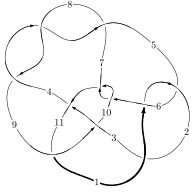
\includegraphics[width=112pt]{../../../GIT/diagram.site/Diagrams/png/417_11a_168.png}\\
\ \ \ A knot diagram\footnotemark}&
\allowdisplaybreaks
\textbf{Linearized knot diagam} \\
\cline{2-2}
 &
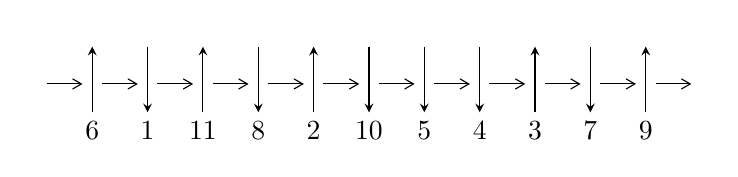
\begin{tikzpicture}[x=20pt, y=17pt]
	% nodes
	\node (C0) at (0, 0) {};
	\node (C1) at (1, 0) {};
	\node (C1U) at (1, +1) {};
	\node (C1D) at (1, -1) {6};

	\node (C2) at (2, 0) {};
	\node (C2U) at (2, +1) {};
	\node (C2D) at (2, -1) {1};

	\node (C3) at (3, 0) {};
	\node (C3U) at (3, +1) {};
	\node (C3D) at (3, -1) {11};

	\node (C4) at (4, 0) {};
	\node (C4U) at (4, +1) {};
	\node (C4D) at (4, -1) {8};

	\node (C5) at (5, 0) {};
	\node (C5U) at (5, +1) {};
	\node (C5D) at (5, -1) {2};

	\node (C6) at (6, 0) {};
	\node (C6U) at (6, +1) {};
	\node (C6D) at (6, -1) {10};

	\node (C7) at (7, 0) {};
	\node (C7U) at (7, +1) {};
	\node (C7D) at (7, -1) {5};

	\node (C8) at (8, 0) {};
	\node (C8U) at (8, +1) {};
	\node (C8D) at (8, -1) {4};

	\node (C9) at (9, 0) {};
	\node (C9U) at (9, +1) {};
	\node (C9D) at (9, -1) {3};

	\node (C10) at (10, 0) {};
	\node (C10U) at (10, +1) {};
	\node (C10D) at (10, -1) {7};

	\node (C11) at (11, 0) {};
	\node (C11U) at (11, +1) {};
	\node (C11D) at (11, -1) {9};
	\node (C12) at (12, 0) {};

	% arrows
	\draw[->,>={angle 60}]
	(C0) edge (C1) (C1) edge (C2) (C2) edge (C3) (C3) edge (C4) (C4) edge (C5) (C5) edge (C6) (C6) edge (C7) (C7) edge (C8) (C8) edge (C9) (C9) edge (C10) (C10) edge (C11) (C11) edge (C12) ;	\draw[->,>=stealth]
	(C1D) edge (C1U) (C2U) edge (C2D) (C3D) edge (C3U) (C4U) edge (C4D) (C5D) edge (C5U) (C6U) edge (C6D) (C7U) edge (C7D) (C8U) edge (C8D) (C9D) edge (C9U) (C10U) edge (C10D) (C11D) edge (C11U) ;
	\end{tikzpicture} \\
\hhline{~~} \\& 
\textbf{Solving Sequence} \\ \cline{2-2} 
 &
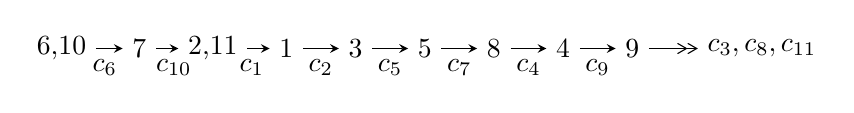
\begin{tikzpicture}[x=25pt, y=7pt]
	% node
	\node (A0) at (-1/8, 0) {6,10};
	\node (A1) at (1, 0) {7};
	\node (A2) at (33/16, 0) {2,11};
	\node (A3) at (25/8, 0) {1};
	\node (A4) at (33/8, 0) {3};
	\node (A5) at (41/8, 0) {5};
	\node (A6) at (49/8, 0) {8};
	\node (A7) at (57/8, 0) {4};
	\node (A8) at (65/8, 0) {9};
	\node (C1) at (1/2, -1) {$c_{6}$};
	\node (C2) at (3/2, -1) {$c_{10}$};
	\node (C3) at (21/8, -1) {$c_{1}$};
	\node (C4) at (29/8, -1) {$c_{2}$};
	\node (C5) at (37/8, -1) {$c_{5}$};
	\node (C6) at (45/8, -1) {$c_{7}$};
	\node (C7) at (53/8, -1) {$c_{4}$};
	\node (C8) at (61/8, -1) {$c_{9}$};
	\node (A9) at (10, 0) {$c_{3},c_{8},c_{11}$};

	% edge
	\draw[->,>=stealth]	
	(A0) edge (A1) (A1) edge (A2) (A2) edge (A3) (A3) edge (A4) (A4) edge (A5) (A5) edge (A6) (A6) edge (A7) (A7) edge (A8) ;
	\draw[->>,>={angle 60}]	
	(A8) edge (A9);
\end{tikzpicture} \\ 

\end{tabular} \\

\footnotetext{
The image of knot diagram is generated by the software ``\textbf{Draw programme}" developed by Andrew Bartholomew(\url{http://www.layer8.co.uk/maths/draw/index.htm\#Running-draw}), where we modified some parts for our purpose(\url{https://github.com/CATsTAILs/LinksPainter}).
}\phantom \\ \newline 
\centering \textbf{Ideals for irreducible components\footnotemark of $X_{\text{par}}$} 
 
\begin{align*}
I^u_{1}&=\langle 
-1.78806\times10^{130} u^{65}-3.53692\times10^{130} u^{64}+\cdots+1.19375\times10^{131} b-9.79607\times10^{131},\\
\phantom{I^u_{1}}&\phantom{= \langle  }-1.13631\times10^{131} u^{65}+6.95957\times10^{131} u^{64}+\cdots+2.74563\times10^{132} a-8.44042\times10^{133},\\
\phantom{I^u_{1}}&\phantom{= \langle  }u^{66}+3 u^{65}+\cdots-49 u+23\rangle \\
I^u_{2}&=\langle 
u^{13}+u^{12}-7 u^{11}-7 u^{10}+19 u^9+21 u^8-26 u^7-35 u^6+19 u^5+33 u^4-4 u^3-18 u^2+b- u+4,\\
\phantom{I^u_{2}}&\phantom{= \langle  }u^{13}+2 u^{12}-5 u^{11}-12 u^{10}+7 u^9+28 u^8+2 u^7-33 u^6-14 u^5+20 u^4+16 u^3-5 u^2+a-5 u,\\
\phantom{I^u_{2}}&\phantom{= \langle  }u^{14}+2 u^{13}-5 u^{12}-12 u^{11}+7 u^{10}+28 u^9+2 u^8-33 u^7-13 u^6+21 u^5+14 u^4-7 u^3-6 u^2+u+1\rangle \\
I^u_{3}&=\langle 
- u^5+2 u^4+u^3-2 u^2+b- u,\;- u^5+2 u^4+a- u,\\
\phantom{I^u_{3}}&\phantom{= \langle  }u^{10}-4 u^9+2 u^8+8 u^7-5 u^6-9 u^5+4 u^4+5 u^3- u^2- u+1\rangle \\
\\
\end{align*}
\raggedright * 3 irreducible components of $\dim_{\mathbb{C}}=0$, with total 90 representations.\\
\footnotetext{All coefficients of polynomials are rational numbers. But the coefficients are sometimes approximated in decimal forms when there is not enough margin.}
\newpage
\renewcommand{\arraystretch}{1}
\centering \section*{I. $I^u_{1}= \langle -1.79\times10^{130} u^{65}-3.54\times10^{130} u^{64}+\cdots+1.19\times10^{131} b-9.80\times10^{131},\;-1.14\times10^{131} u^{65}+6.96\times10^{131} u^{64}+\cdots+2.75\times10^{132} a-8.44\times10^{133},\;u^{66}+3 u^{65}+\cdots-49 u+23 \rangle$}
\flushleft \textbf{(i) Arc colorings}\\
\begin{tabular}{m{7pt} m{180pt} m{7pt} m{180pt} }
\flushright $a_{6}=$&$\begin{pmatrix}1\\0\end{pmatrix}$ \\
\flushright $a_{10}=$&$\begin{pmatrix}0\\u\end{pmatrix}$ \\
\flushright $a_{7}=$&$\begin{pmatrix}1\\u^2\end{pmatrix}$ \\
\flushright $a_{2}=$&$\begin{pmatrix}0.0413863 u^{65}-0.253478 u^{64}+\cdots-71.6967 u+30.7413\\0.149785 u^{65}+0.296286 u^{64}+\cdots-25.4119 u+8.20610\end{pmatrix}$ \\
\flushright $a_{11}=$&$\begin{pmatrix}- u\\- u^3+u\end{pmatrix}$ \\
\flushright $a_{1}=$&$\begin{pmatrix}-0.108398 u^{65}-0.549764 u^{64}+\cdots-46.2848 u+22.5351\\0.149785 u^{65}+0.296286 u^{64}+\cdots-25.4119 u+8.20610\end{pmatrix}$ \\
\flushright $a_{3}=$&$\begin{pmatrix}-0.265019 u^{65}-0.684530 u^{64}+\cdots+16.5444 u-1.80031\\0.0970785 u^{65}+0.246976 u^{64}+\cdots-17.2639 u+5.68359\end{pmatrix}$ \\
\flushright $a_{5}=$&$\begin{pmatrix}0.0633462 u^{65}+0.131815 u^{64}+\cdots+22.7802 u-6.63331\\0.0144495 u^{65}+0.0765866 u^{64}+\cdots+23.6745 u-8.68302\end{pmatrix}$ \\
\flushright $a_{8}=$&$\begin{pmatrix}0.241521 u^{65}+0.174805 u^{64}+\cdots-90.4271 u+35.3903\\0.0842047 u^{65}+0.187816 u^{64}+\cdots-24.7015 u+6.71251\end{pmatrix}$ \\
\flushright $a_{4}=$&$\begin{pmatrix}-0.352721 u^{65}-0.894904 u^{64}+\cdots+18.6230 u-2.09481\\0.119566 u^{65}+0.307098 u^{64}+\cdots-14.7416 u+4.76525\end{pmatrix}$ \\
\flushright $a_{9}=$&$\begin{pmatrix}-0.204510 u^{65}-0.292070 u^{64}+\cdots+36.4550 u-17.5683\\0.00530887 u^{65}+0.0353219 u^{64}+\cdots+5.95418 u-2.01143\end{pmatrix}$\\ \flushright $a_{9}=$&$\begin{pmatrix}-0.204510 u^{65}-0.292070 u^{64}+\cdots+36.4550 u-17.5683\\0.00530887 u^{65}+0.0353219 u^{64}+\cdots+5.95418 u-2.01143\end{pmatrix}$\\&\end{tabular}
\flushleft \textbf{(ii) Obstruction class $= -1$}\\~\\
\flushleft \textbf{(iii) Cusp Shapes $= 1.39895 u^{65}+3.59121 u^{64}+\cdots-107.584 u+25.1145$}\\~\\
\newpage\renewcommand{\arraystretch}{1}
\flushleft \textbf{(iv) u-Polynomials at the component}\newline \\
\begin{tabular}{m{50pt}|m{274pt}}
Crossings & \hspace{64pt}u-Polynomials at each crossing \\
\hline $$\begin{aligned}c_{1},c_{5}\end{aligned}$$&$\begin{aligned}
&u^{66}+5 u^{65}+\cdots+70 u+28
\end{aligned}$\\
\hline $$\begin{aligned}c_{2}\end{aligned}$$&$\begin{aligned}
&u^{66}+27 u^{65}+\cdots+5684 u+784
\end{aligned}$\\
\hline $$\begin{aligned}c_{3}\end{aligned}$$&$\begin{aligned}
&u^{66}+7 u^{65}+\cdots-293 u+131
\end{aligned}$\\
\hline $$\begin{aligned}c_{4},c_{7},c_{8}\end{aligned}$$&$\begin{aligned}
&u^{66}-2 u^{65}+\cdots-20 u+1
\end{aligned}$\\
\hline $$\begin{aligned}c_{6},c_{10}\end{aligned}$$&$\begin{aligned}
&u^{66}+3 u^{65}+\cdots-49 u+23
\end{aligned}$\\
\hline $$\begin{aligned}c_{9}\end{aligned}$$&$\begin{aligned}
&u^{66}+2 u^{64}+\cdots+24 u+1
\end{aligned}$\\
\hline $$\begin{aligned}c_{11}\end{aligned}$$&$\begin{aligned}
&u^{66}+5 u^{65}+\cdots+3276 u+667
\end{aligned}$\\
\hline
\end{tabular}\\~\\
\newpage\renewcommand{\arraystretch}{1}
\flushleft \textbf{(v) Riley Polynomials at the component}\newline \\
\begin{tabular}{m{50pt}|m{274pt}}
Crossings & \hspace{64pt}Riley Polynomials at each crossing \\
\hline $$\begin{aligned}c_{1},c_{5}\end{aligned}$$&$\begin{aligned}
&y^{66}+27 y^{65}+\cdots+5684 y+784
\end{aligned}$\\
\hline $$\begin{aligned}c_{2}\end{aligned}$$&$\begin{aligned}
&y^{66}+27 y^{65}+\cdots+5306896 y+614656
\end{aligned}$\\
\hline $$\begin{aligned}c_{3}\end{aligned}$$&$\begin{aligned}
&y^{66}-15 y^{65}+\cdots-380599 y+17161
\end{aligned}$\\
\hline $$\begin{aligned}c_{4},c_{7},c_{8}\end{aligned}$$&$\begin{aligned}
&y^{66}+72 y^{65}+\cdots-2 y+1
\end{aligned}$\\
\hline $$\begin{aligned}c_{6},c_{10}\end{aligned}$$&$\begin{aligned}
&y^{66}-33 y^{65}+\cdots-12015 y+529
\end{aligned}$\\
\hline $$\begin{aligned}c_{9}\end{aligned}$$&$\begin{aligned}
&y^{66}+4 y^{65}+\cdots-30 y+1
\end{aligned}$\\
\hline $$\begin{aligned}c_{11}\end{aligned}$$&$\begin{aligned}
&y^{66}-15 y^{65}+\cdots-11892756 y+444889
\end{aligned}$\\
\hline
\end{tabular}\\~\\
\newpage\flushleft \textbf{(vi) Complex Volumes and Cusp Shapes}
$$\begin{array}{c|c|c}  
\text{Solutions to }I^u_{1}& \I (\text{vol} + \sqrt{-1}CS) & \text{Cusp shape}\\
 \hline 
\begin{aligned}
u &= \phantom{-}0.163567 + 0.974073 I \\
a &= \phantom{-}0.696136 - 0.268743 I \\
b &= -0.580597 - 1.004650 I\end{aligned}
 & \phantom{-}1.17857 + 6.31445 I & \phantom{-0.000000 } 0. - 8.26296 I \\ \hline\begin{aligned}
u &= \phantom{-}0.163567 - 0.974073 I \\
a &= \phantom{-}0.696136 + 0.268743 I \\
b &= -0.580597 + 1.004650 I\end{aligned}
 & \phantom{-}1.17857 - 6.31445 I & \phantom{-0.000000 -}0. + 8.26296 I \\ \hline\begin{aligned}
u &= -0.910079 + 0.369691 I \\
a &= \phantom{-}0.303793 - 0.056648 I \\
b &= -0.458628 + 0.318939 I\end{aligned}
 & -1.48654 + 0.69916 I & -4.61313 - 2.12935 I \\ \hline\begin{aligned}
u &= -0.910079 - 0.369691 I \\
a &= \phantom{-}0.303793 + 0.056648 I \\
b &= -0.458628 - 0.318939 I\end{aligned}
 & -1.48654 - 0.69916 I & -4.61313 + 2.12935 I \\ \hline\begin{aligned}
u &= \phantom{-}0.975903 + 0.320029 I \\
a &= -0.65293 - 2.09713 I \\
b &= \phantom{-}0.603233 - 1.184400 I\end{aligned}
 & -1.41728 - 5.05455 I & \phantom{-0.000000 -}0. + 12.20236 I \\ \hline\begin{aligned}
u &= \phantom{-}0.975903 - 0.320029 I \\
a &= -0.65293 + 2.09713 I \\
b &= \phantom{-}0.603233 + 1.184400 I\end{aligned}
 & -1.41728 + 5.05455 I & \phantom{-0.000000 } 0. - 12.20236 I \\ \hline\begin{aligned}
u &= -0.881923 + 0.307874 I \\
a &= -0.200444 + 0.477752 I \\
b &= \phantom{-}0.744898 - 0.630242 I\end{aligned}
 & \phantom{-}0.032145 + 0.573668 I & \phantom{-0.000000 } 0. - 4.06060 I \\ \hline\begin{aligned}
u &= -0.881923 - 0.307874 I \\
a &= -0.200444 - 0.477752 I \\
b &= \phantom{-}0.744898 + 0.630242 I\end{aligned}
 & \phantom{-}0.032145 - 0.573668 I & \phantom{-0.000000 -}0. + 4.06060 I \\ \hline\begin{aligned}
u &= -0.950720 + 0.502350 I \\
a &= -0.877967 + 0.026202 I \\
b &= -1.016380 + 0.270524 I\end{aligned}
 & \phantom{-}6.72384 - 0.00894 I & \phantom{-0.000000 } 0 \\ \hline\begin{aligned}
u &= -0.950720 - 0.502350 I \\
a &= -0.877967 - 0.026202 I \\
b &= -1.016380 - 0.270524 I\end{aligned}
 & \phantom{-}6.72384 + 0.00894 I & \phantom{-0.000000 } 0\\
 \hline 
 \end{array}$$\newpage$$\begin{array}{c|c|c}  
\text{Solutions to }I^u_{1}& \I (\text{vol} + \sqrt{-1}CS) & \text{Cusp shape}\\
 \hline 
\begin{aligned}
u &= \phantom{-}0.895747 + 0.113324 I \\
a &= -0.210467 - 0.615238 I \\
b &= \phantom{-}0.723006 - 0.613380 I\end{aligned}
 & \phantom{-}0.35093 - 2.50495 I & \phantom{-}1.76854 + 6.87309 I \\ \hline\begin{aligned}
u &= \phantom{-}0.895747 - 0.113324 I \\
a &= -0.210467 + 0.615238 I \\
b &= \phantom{-}0.723006 + 0.613380 I\end{aligned}
 & \phantom{-}0.35093 + 2.50495 I & \phantom{-}1.76854 - 6.87309 I \\ \hline\begin{aligned}
u &= \phantom{-}0.513355 + 0.969879 I \\
a &= -0.554489 - 0.295569 I \\
b &= \phantom{-}0.061422 + 0.772480 I\end{aligned}
 & \phantom{-}3.81529 - 4.03349 I & \phantom{-0.000000 } 0 \\ \hline\begin{aligned}
u &= \phantom{-}0.513355 - 0.969879 I \\
a &= -0.554489 + 0.295569 I \\
b &= \phantom{-}0.061422 - 0.772480 I\end{aligned}
 & \phantom{-}3.81529 + 4.03349 I & \phantom{-0.000000 } 0 \\ \hline\begin{aligned}
u &= -1.003490 + 0.462245 I \\
a &= -1.38592 + 1.18971 I \\
b &= \phantom{-}0.658324 + 1.027690 I\end{aligned}
 & -1.18063 + 5.94761 I & \phantom{-0.000000 } 0 \\ \hline\begin{aligned}
u &= -1.003490 - 0.462245 I \\
a &= -1.38592 - 1.18971 I \\
b &= \phantom{-}0.658324 - 1.027690 I\end{aligned}
 & -1.18063 - 5.94761 I & \phantom{-0.000000 } 0 \\ \hline\begin{aligned}
u &= \phantom{-}0.213343 + 0.781690 I \\
a &= \phantom{-}1.040630 + 0.205621 I \\
b &= -0.630515 + 0.547682 I\end{aligned}
 & \phantom{-}2.50610 + 1.55549 I & \phantom{-}4.46271 - 2.30891 I \\ \hline\begin{aligned}
u &= \phantom{-}0.213343 - 0.781690 I \\
a &= \phantom{-}1.040630 - 0.205621 I \\
b &= -0.630515 - 0.547682 I\end{aligned}
 & \phantom{-}2.50610 - 1.55549 I & \phantom{-}4.46271 + 2.30891 I \\ \hline\begin{aligned}
u &= -0.435912 + 0.662170 I \\
a &= \phantom{-}0.380983 + 0.238349 I \\
b &= -0.160229 + 0.802581 I\end{aligned}
 & -1.40850 + 1.04300 I & -5.70485 - 4.49521 I \\ \hline\begin{aligned}
u &= -0.435912 - 0.662170 I \\
a &= \phantom{-}0.380983 - 0.238349 I \\
b &= -0.160229 - 0.802581 I\end{aligned}
 & -1.40850 - 1.04300 I & -5.70485 + 4.49521 I\\
 \hline 
 \end{array}$$\newpage$$\begin{array}{c|c|c}  
\text{Solutions to }I^u_{1}& \I (\text{vol} + \sqrt{-1}CS) & \text{Cusp shape}\\
 \hline 
\begin{aligned}
u &= -1.142840 + 0.408088 I \\
a &= \phantom{-}0.12099 - 2.00122 I \\
b &= -0.017416 - 1.388480 I\end{aligned}
 & -0.42442 + 7.17415 I & \phantom{-0.000000 } 0 \\ \hline\begin{aligned}
u &= -1.142840 - 0.408088 I \\
a &= \phantom{-}0.12099 + 2.00122 I \\
b &= -0.017416 + 1.388480 I\end{aligned}
 & -0.42442 - 7.17415 I & \phantom{-0.000000 } 0 \\ \hline\begin{aligned}
u &= \phantom{-}1.120610 + 0.507476 I \\
a &= -0.213239 + 0.187929 I \\
b &= -0.870327 - 0.488823 I\end{aligned}
 & -0.11868 - 6.20190 I & \phantom{-0.000000 } 0 \\ \hline\begin{aligned}
u &= \phantom{-}1.120610 - 0.507476 I \\
a &= -0.213239 - 0.187929 I \\
b &= -0.870327 + 0.488823 I\end{aligned}
 & -0.11868 + 6.20190 I & \phantom{-0.000000 } 0 \\ \hline\begin{aligned}
u &= \phantom{-}0.348013 + 0.685297 I \\
a &= \phantom{-}0.385405 + 0.184638 I \\
b &= -0.782208 + 0.911468 I\end{aligned}
 & \phantom{-}8.00774 - 2.72139 I & \phantom{-}5.67340 + 3.59670 I \\ \hline\begin{aligned}
u &= \phantom{-}0.348013 - 0.685297 I \\
a &= \phantom{-}0.385405 - 0.184638 I \\
b &= -0.782208 - 0.911468 I\end{aligned}
 & \phantom{-}8.00774 + 2.72139 I & \phantom{-}5.67340 - 3.59670 I \\ \hline\begin{aligned}
u &= \phantom{-}1.174490 + 0.439061 I \\
a &= \phantom{-}0.55437 + 2.35095 I \\
b &= -0.581613 + 0.937637 I\end{aligned}
 & \phantom{-}5.38489 - 7.07352 I & \phantom{-0.000000 } 0 \\ \hline\begin{aligned}
u &= \phantom{-}1.174490 - 0.439061 I \\
a &= \phantom{-}0.55437 - 2.35095 I \\
b &= -0.581613 - 0.937637 I\end{aligned}
 & \phantom{-}5.38489 + 7.07352 I & \phantom{-0.000000 } 0 \\ \hline\begin{aligned}
u &= \phantom{-}1.082830 + 0.650499 I \\
a &= -0.763412 - 0.125255 I \\
b &= -0.584235 - 0.734442 I\end{aligned}
 & \phantom{-}6.02312 - 2.42646 I & \phantom{-0.000000 } 0 \\ \hline\begin{aligned}
u &= \phantom{-}1.082830 - 0.650499 I \\
a &= -0.763412 + 0.125255 I \\
b &= -0.584235 + 0.734442 I\end{aligned}
 & \phantom{-}6.02312 + 2.42646 I & \phantom{-0.000000 } 0\\
 \hline 
 \end{array}$$\newpage$$\begin{array}{c|c|c}  
\text{Solutions to }I^u_{1}& \I (\text{vol} + \sqrt{-1}CS) & \text{Cusp shape}\\
 \hline 
\begin{aligned}
u &= \phantom{-}1.240570 + 0.249436 I \\
a &= -0.25707 - 1.89384 I \\
b &= -0.025398 - 1.232230 I\end{aligned}
 & -6.29461 - 3.96507 I & \phantom{-0.000000 } 0 \\ \hline\begin{aligned}
u &= \phantom{-}1.240570 - 0.249436 I \\
a &= -0.25707 + 1.89384 I \\
b &= -0.025398 + 1.232230 I\end{aligned}
 & -6.29461 + 3.96507 I & \phantom{-0.000000 } 0 \\ \hline\begin{aligned}
u &= -0.456533 + 1.193620 I \\
a &= -0.479732 + 0.721690 I \\
b &= \phantom{-}0.787442 + 0.623044 I\end{aligned}
 & \phantom{-}9.11482 - 3.60155 I & \phantom{-0.000000 } 0 \\ \hline\begin{aligned}
u &= -0.456533 - 1.193620 I \\
a &= -0.479732 - 0.721690 I \\
b &= \phantom{-}0.787442 - 0.623044 I\end{aligned}
 & \phantom{-}9.11482 + 3.60155 I & \phantom{-0.000000 } 0 \\ \hline\begin{aligned}
u &= \phantom{-}0.970943 + 0.846933 I \\
a &= -0.110406 - 0.251793 I \\
b &= \phantom{-}0.601898 + 0.133589 I\end{aligned}
 & \phantom{-}3.63388 - 3.20673 I & \phantom{-0.000000 } 0 \\ \hline\begin{aligned}
u &= \phantom{-}0.970943 - 0.846933 I \\
a &= -0.110406 + 0.251793 I \\
b &= \phantom{-}0.601898 - 0.133589 I\end{aligned}
 & \phantom{-}3.63388 + 3.20673 I & \phantom{-0.000000 } 0 \\ \hline\begin{aligned}
u &= -1.233540 + 0.392626 I \\
a &= \phantom{-}0.21257 - 2.00569 I \\
b &= -0.71720 - 1.24384 I\end{aligned}
 & \phantom{-}3.82726 + 6.26660 I & \phantom{-0.000000 } 0 \\ \hline\begin{aligned}
u &= -1.233540 - 0.392626 I \\
a &= \phantom{-}0.21257 + 2.00569 I \\
b &= -0.71720 + 1.24384 I\end{aligned}
 & \phantom{-}3.82726 - 6.26660 I & \phantom{-0.000000 } 0 \\ \hline\begin{aligned}
u &= -1.317410 + 0.143765 I \\
a &= \phantom{-}0.58844 - 1.71642 I \\
b &= \phantom{-}0.100771 - 0.992542 I\end{aligned}
 & -4.86658 + 0.02437 I & \phantom{-0.000000 } 0 \\ \hline\begin{aligned}
u &= -1.317410 - 0.143765 I \\
a &= \phantom{-}0.58844 + 1.71642 I \\
b &= \phantom{-}0.100771 + 0.992542 I\end{aligned}
 & -4.86658 - 0.02437 I & \phantom{-0.000000 } 0\\
 \hline 
 \end{array}$$\newpage$$\begin{array}{c|c|c}  
\text{Solutions to }I^u_{1}& \I (\text{vol} + \sqrt{-1}CS) & \text{Cusp shape}\\
 \hline 
\begin{aligned}
u &= -0.599634 + 0.293642 I \\
a &= -0.360866 - 1.059790 I \\
b &= -1.107300 - 0.801620 I\end{aligned}
 & \phantom{-}7.97540 + 3.77535 I & \phantom{-}12.7373 - 9.7511 I \\ \hline\begin{aligned}
u &= -0.599634 - 0.293642 I \\
a &= -0.360866 + 1.059790 I \\
b &= -1.107300 + 0.801620 I\end{aligned}
 & \phantom{-}7.97540 - 3.77535 I & \phantom{-}12.7373 + 9.7511 I \\ \hline\begin{aligned}
u &= \phantom{-}1.189390 + 0.620718 I \\
a &= -0.11891 + 1.45206 I \\
b &= \phantom{-}0.333461 + 1.110410 I\end{aligned}
 & \phantom{-}0.1230110 + 0.0150349 I & \phantom{-0.000000 } 0 \\ \hline\begin{aligned}
u &= \phantom{-}1.189390 - 0.620718 I \\
a &= -0.11891 - 1.45206 I \\
b &= \phantom{-}0.333461 - 1.110410 I\end{aligned}
 & \phantom{-}0.1230110 - 0.0150349 I & \phantom{-0.000000 } 0 \\ \hline\begin{aligned}
u &= \phantom{-}1.229960 + 0.588843 I \\
a &= \phantom{-}0.98305 + 1.56765 I \\
b &= -0.665256 + 1.110210 I\end{aligned}
 & -1.99580 - 11.89200 I & \phantom{-0.000000 } 0 \\ \hline\begin{aligned}
u &= \phantom{-}1.229960 - 0.588843 I \\
a &= \phantom{-}0.98305 - 1.56765 I \\
b &= -0.665256 - 1.110210 I\end{aligned}
 & -1.99580 + 11.89200 I & \phantom{-0.000000 } 0 \\ \hline\begin{aligned}
u &= \phantom{-}0.626363 + 0.088665 I \\
a &= \phantom{-}2.69216 - 3.52949 I \\
b &= -0.309304 - 0.848107 I\end{aligned}
 & \phantom{-}3.63938 - 2.52827 I & -1.147337 - 0.754292 I \\ \hline\begin{aligned}
u &= \phantom{-}0.626363 - 0.088665 I \\
a &= \phantom{-}2.69216 + 3.52949 I \\
b &= -0.309304 + 0.848107 I\end{aligned}
 & \phantom{-}3.63938 + 2.52827 I & -1.147337 + 0.754292 I \\ \hline\begin{aligned}
u &= -1.218200 + 0.688747 I \\
a &= \phantom{-}0.95882 - 1.32677 I \\
b &= -0.514831 - 1.018630 I\end{aligned}
 & -3.18756 + 4.76965 I & \phantom{-0.000000 } 0 \\ \hline\begin{aligned}
u &= -1.218200 - 0.688747 I \\
a &= \phantom{-}0.95882 + 1.32677 I \\
b &= -0.514831 + 1.018630 I\end{aligned}
 & -3.18756 - 4.76965 I & \phantom{-0.000000 } 0\\
 \hline 
 \end{array}$$\newpage$$\begin{array}{c|c|c}  
\text{Solutions to }I^u_{1}& \I (\text{vol} + \sqrt{-1}CS) & \text{Cusp shape}\\
 \hline 
\begin{aligned}
u &= -0.582346 + 0.119440 I \\
a &= \phantom{-}0.65201 + 3.57882 I \\
b &= -0.423495 + 1.216100 I\end{aligned}
 & \phantom{-}2.04523 - 4.42740 I & \phantom{-}0.06553 + 3.55579 I \\ \hline\begin{aligned}
u &= -0.582346 - 0.119440 I \\
a &= \phantom{-}0.65201 - 3.57882 I \\
b &= -0.423495 - 1.216100 I\end{aligned}
 & \phantom{-}2.04523 + 4.42740 I & \phantom{-}0.06553 - 3.55579 I \\ \hline\begin{aligned}
u &= -1.214820 + 0.714561 I \\
a &= \phantom{-}0.338561 + 0.013564 I \\
b &= \phantom{-}0.986535 - 0.471169 I\end{aligned}
 & \phantom{-}6.64257 + 10.26800 I & \phantom{-0.000000 } 0 \\ \hline\begin{aligned}
u &= -1.214820 - 0.714561 I \\
a &= \phantom{-}0.338561 - 0.013564 I \\
b &= \phantom{-}0.986535 + 0.471169 I\end{aligned}
 & \phantom{-}6.64257 - 10.26800 I & \phantom{-0.000000 } 0 \\ \hline\begin{aligned}
u &= -0.29930 + 1.39073 I \\
a &= -0.274401 - 0.646909 I \\
b &= \phantom{-}0.664803 - 1.023810 I\end{aligned}
 & \phantom{-}7.89254 - 9.07916 I & \phantom{-0.000000 } 0 \\ \hline\begin{aligned}
u &= -0.29930 - 1.39073 I \\
a &= -0.274401 + 0.646909 I \\
b &= \phantom{-}0.664803 + 1.023810 I\end{aligned}
 & \phantom{-}7.89254 + 9.07916 I & \phantom{-0.000000 } 0 \\ \hline\begin{aligned}
u &= \phantom{-}0.477375 + 0.237133 I \\
a &= \phantom{-}1.096490 - 0.505493 I \\
b &= \phantom{-}0.681358 + 0.179083 I\end{aligned}
 & \phantom{-}1.48045 + 0.06659 I & \phantom{-}8.57715 + 1.33589 I \\ \hline\begin{aligned}
u &= \phantom{-}0.477375 - 0.237133 I \\
a &= \phantom{-}1.096490 + 0.505493 I \\
b &= \phantom{-}0.681358 - 0.179083 I\end{aligned}
 & \phantom{-}1.48045 - 0.06659 I & \phantom{-}8.57715 - 1.33589 I \\ \hline\begin{aligned}
u &= -1.51195 + 0.21374 I \\
a &= \phantom{-}0.104633 + 1.369450 I \\
b &= -0.342184 + 0.961816 I\end{aligned}
 & -4.43757 - 1.23820 I & \phantom{-0.000000 } 0 \\ \hline\begin{aligned}
u &= -1.51195 - 0.21374 I \\
a &= \phantom{-}0.104633 - 1.369450 I \\
b &= -0.342184 - 0.961816 I\end{aligned}
 & -4.43757 + 1.23820 I & \phantom{-0.000000 } 0\\
 \hline 
 \end{array}$$\newpage$$\begin{array}{c|c|c}  
\text{Solutions to }I^u_{1}& \I (\text{vol} + \sqrt{-1}CS) & \text{Cusp shape}\\
 \hline 
\begin{aligned}
u &= -1.34952 + 0.73556 I \\
a &= -0.72074 + 1.63019 I \\
b &= \phantom{-}0.695108 + 1.158380 I\end{aligned}
 & \phantom{-}4.5173 + 16.3689 I & \phantom{-0.000000 } 0 \\ \hline\begin{aligned}
u &= -1.34952 - 0.73556 I \\
a &= -0.72074 - 1.63019 I \\
b &= \phantom{-}0.695108 - 1.158380 I\end{aligned}
 & \phantom{-}4.5173 - 16.3689 I & \phantom{-0.000000 } 0 \\ \hline\begin{aligned}
u &= \phantom{-}1.13836 + 1.03918 I \\
a &= -0.99274 - 1.43051 I \\
b &= \phantom{-}0.496265 - 1.089620 I\end{aligned}
 & \phantom{-}1.16169 - 7.37354 I & \phantom{-0.000000 } 0 \\ \hline\begin{aligned}
u &= \phantom{-}1.13836 - 1.03918 I \\
a &= -0.99274 + 1.43051 I \\
b &= \phantom{-}0.496265 + 1.089620 I\end{aligned}
 & \phantom{-}1.16169 + 7.37354 I & \phantom{-0.000000 } 0 \\ \hline\begin{aligned}
u &= \phantom{-}0.247407 + 0.342006 I \\
a &= \phantom{-}1.23861 - 0.86436 I \\
b &= -0.851416 - 0.882734 I\end{aligned}
 & \phantom{-}8.18428 + 3.39136 I & \phantom{-}6.60752 + 1.70089 I \\ \hline\begin{aligned}
u &= \phantom{-}0.247407 - 0.342006 I \\
a &= \phantom{-}1.23861 + 0.86436 I \\
b &= -0.851416 + 0.882734 I\end{aligned}
 & \phantom{-}8.18428 - 3.39136 I & \phantom{-}6.60752 - 1.70089 I\\
 \hline 
 \end{array}$$\newpage\newpage\renewcommand{\arraystretch}{1}
\centering \section*{II. $I^u_{2}= \langle u^{13}+u^{12}+\cdots+b+4,\;u^{13}+2 u^{12}+\cdots+a-5 u,\;u^{14}+2 u^{13}+\cdots+u+1 \rangle$}
\flushleft \textbf{(i) Arc colorings}\\
\begin{tabular}{m{7pt} m{180pt} m{7pt} m{180pt} }
\flushright $a_{6}=$&$\begin{pmatrix}1\\0\end{pmatrix}$ \\
\flushright $a_{10}=$&$\begin{pmatrix}0\\u\end{pmatrix}$ \\
\flushright $a_{7}=$&$\begin{pmatrix}1\\u^2\end{pmatrix}$ \\
\flushright $a_{2}=$&$\begin{pmatrix}- u^{13}-2 u^{12}+\cdots+5 u^2+5 u\\- u^{13}- u^{12}+\cdots+u-4\end{pmatrix}$ \\
\flushright $a_{11}=$&$\begin{pmatrix}- u\\- u^3+u\end{pmatrix}$ \\
\flushright $a_{1}=$&$\begin{pmatrix}- u^{12}-2 u^{11}+\cdots+4 u+4\\- u^{13}- u^{12}+\cdots+u-4\end{pmatrix}$ \\
\flushright $a_{3}=$&$\begin{pmatrix}u^{13}+u^{12}+\cdots+5 u+4\\-4 u^{13}-4 u^{12}+\cdots+51 u^2-10\end{pmatrix}$ \\
\flushright $a_{5}=$&$\begin{pmatrix}2 u^{13}+4 u^{12}+\cdots-8 u^2+3\\4 u^{13}+7 u^{12}+\cdots-6 u+4\end{pmatrix}$ \\
\flushright $a_{8}=$&$\begin{pmatrix}2 u^{13}+3 u^{12}+\cdots-4 u+2\\- u^{12}- u^{11}+\cdots+5 u-1\end{pmatrix}$ \\
\flushright $a_{4}=$&$\begin{pmatrix}u^{11}+2 u^{10}+\cdots+6 u+1\\-3 u^{13}-3 u^{12}+\cdots- u-8\end{pmatrix}$ \\
\flushright $a_{9}=$&$\begin{pmatrix}u^{12}+2 u^{11}+\cdots-6 u-5\\u^{13}+u^{12}+\cdots-20 u^2+5\end{pmatrix}$\\ \flushright $a_{9}=$&$\begin{pmatrix}u^{12}+2 u^{11}+\cdots-6 u-5\\u^{13}+u^{12}+\cdots-20 u^2+5\end{pmatrix}$\\&\end{tabular}
\flushleft \textbf{(ii) Obstruction class $= 1$}\\~\\
\flushleft \textbf{(iii) Cusp Shapes $= -4 u^{13}-9 u^{12}+20 u^{11}+56 u^{10}-28 u^9-137 u^8-11 u^7+169 u^6+61 u^5-113 u^4-60 u^3+42 u^2+22 u-10$}\\~\\
\newpage\renewcommand{\arraystretch}{1}
\flushleft \textbf{(iv) u-Polynomials at the component}\newline \\
\begin{tabular}{m{50pt}|m{274pt}}
Crossings & \hspace{64pt}u-Polynomials at each crossing \\
\hline $$\begin{aligned}c_{1}\end{aligned}$$&$\begin{aligned}
&u^{14}- u^{13}+\cdots+4 u^2+1
\end{aligned}$\\
\hline $$\begin{aligned}c_{2}\end{aligned}$$&$\begin{aligned}
&u^{14}+7 u^{13}+\cdots+8 u+1
\end{aligned}$\\
\hline $$\begin{aligned}c_{3}\end{aligned}$$&$\begin{aligned}
&u^{14}+2 u^{11}-2 u^{10}- u^9- u^8-2 u^7+4 u^6+2 u^5-2 u^3- u+1
\end{aligned}$\\
\hline $$\begin{aligned}c_{4}\end{aligned}$$&$\begin{aligned}
&u^{14}- u^{13}+\cdots+4 u^2+1
\end{aligned}$\\
\hline $$\begin{aligned}c_{5}\end{aligned}$$&$\begin{aligned}
&u^{14}+u^{13}+\cdots+4 u^2+1
\end{aligned}$\\
\hline $$\begin{aligned}c_{6}\end{aligned}$$&$\begin{aligned}
&u^{14}+2 u^{13}+\cdots+u+1
\end{aligned}$\\
\hline $$\begin{aligned}c_{7},c_{8}\end{aligned}$$&$\begin{aligned}
&u^{14}+u^{13}+\cdots+4 u^2+1
\end{aligned}$\\
\hline $$\begin{aligned}c_{9}\end{aligned}$$&$\begin{aligned}
&u^{14}+u^{13}+2 u^{11}-2 u^9+4 u^8+2 u^7- u^6+u^5-2 u^4-2 u^3+1
\end{aligned}$\\
\hline $$\begin{aligned}c_{10}\end{aligned}$$&$\begin{aligned}
&u^{14}-2 u^{13}+\cdots- u+1
\end{aligned}$\\
\hline $$\begin{aligned}c_{11}\end{aligned}$$&$\begin{aligned}
&u^{14}-4 u^{12}+\cdots-6 u+1
\end{aligned}$\\
\hline
\end{tabular}\\~\\
\newpage\renewcommand{\arraystretch}{1}
\flushleft \textbf{(v) Riley Polynomials at the component}\newline \\
\begin{tabular}{m{50pt}|m{274pt}}
Crossings & \hspace{64pt}Riley Polynomials at each crossing \\
\hline $$\begin{aligned}c_{1},c_{5}\end{aligned}$$&$\begin{aligned}
&y^{14}+7 y^{13}+\cdots+8 y+1
\end{aligned}$\\
\hline $$\begin{aligned}c_{2}\end{aligned}$$&$\begin{aligned}
&y^{14}+7 y^{13}+\cdots+4 y+1
\end{aligned}$\\
\hline $$\begin{aligned}c_{3}\end{aligned}$$&$\begin{aligned}
&y^{14}-4 y^{12}+\cdots- y+1
\end{aligned}$\\
\hline $$\begin{aligned}c_{4},c_{7},c_{8}\end{aligned}$$&$\begin{aligned}
&y^{14}+15 y^{13}+\cdots+8 y+1
\end{aligned}$\\
\hline $$\begin{aligned}c_{6},c_{10}\end{aligned}$$&$\begin{aligned}
&y^{14}-14 y^{13}+\cdots-13 y+1
\end{aligned}$\\
\hline $$\begin{aligned}c_{9}\end{aligned}$$&$\begin{aligned}
&y^{14}- y^{13}+\cdots-4 y^2+1
\end{aligned}$\\
\hline $$\begin{aligned}c_{11}\end{aligned}$$&$\begin{aligned}
&y^{14}-8 y^{13}+\cdots-6 y+1
\end{aligned}$\\
\hline
\end{tabular}\\~\\
\newpage\flushleft \textbf{(vi) Complex Volumes and Cusp Shapes}
$$\begin{array}{c|c|c}  
\text{Solutions to }I^u_{2}& \I (\text{vol} + \sqrt{-1}CS) & \text{Cusp shape}\\
 \hline 
\begin{aligned}
u &= \phantom{-}0.893293 + 0.330555 I \\
a &= -1.15727 - 1.80484 I \\
b &= \phantom{-}0.592535 - 1.077080 I\end{aligned}
 & -1.31269 - 4.25298 I & -1.95653 + 2.08128 I \\ \hline\begin{aligned}
u &= \phantom{-}0.893293 - 0.330555 I \\
a &= -1.15727 + 1.80484 I \\
b &= \phantom{-}0.592535 + 1.077080 I\end{aligned}
 & -1.31269 + 4.25298 I & -1.95653 - 2.08128 I \\ \hline\begin{aligned}
u &= -0.647670 + 0.662108 I \\
a &= -0.510220 - 1.279880 I \\
b &= -0.233748 + 0.627547 I\end{aligned}
 & \phantom{-}4.41438 + 3.29645 I & \phantom{-}4.47890 - 2.20670 I \\ \hline\begin{aligned}
u &= -0.647670 - 0.662108 I \\
a &= -0.510220 + 1.279880 I \\
b &= -0.233748 - 0.627547 I\end{aligned}
 & \phantom{-}4.41438 - 3.29645 I & \phantom{-}4.47890 + 2.20670 I \\ \hline\begin{aligned}
u &= -1.004110 + 0.573368 I \\
a &= \phantom{-}0.83903 - 2.27992 I \\
b &= -0.459822 - 1.169450 I\end{aligned}
 & \phantom{-}2.10465 + 6.34173 I & \phantom{-}0.34884 - 6.28453 I \\ \hline\begin{aligned}
u &= -1.004110 - 0.573368 I \\
a &= \phantom{-}0.83903 + 2.27992 I \\
b &= -0.459822 + 1.169450 I\end{aligned}
 & \phantom{-}2.10465 - 6.34173 I & \phantom{-}0.34884 + 6.28453 I \\ \hline\begin{aligned}
u &= \phantom{-}0.630522 + 0.153615 I \\
a &= \phantom{-}0.851195 - 1.013010 I \\
b &= \phantom{-}0.557304 + 0.531416 I\end{aligned}
 & \phantom{-}0.482214 + 0.495105 I & \phantom{-}1.13492 - 1.08750 I \\ \hline\begin{aligned}
u &= \phantom{-}0.630522 - 0.153615 I \\
a &= \phantom{-}0.851195 + 1.013010 I \\
b &= \phantom{-}0.557304 - 0.531416 I\end{aligned}
 & \phantom{-}0.482214 - 0.495105 I & \phantom{-}1.13492 + 1.08750 I \\ \hline\begin{aligned}
u &= -0.599098 + 0.137170 I \\
a &= -0.253842 - 0.494489 I \\
b &= -1.007620 - 0.852501 I\end{aligned}
 & \phantom{-}7.61522 + 3.62847 I & -8.05550 - 2.25038 I \\ \hline\begin{aligned}
u &= -0.599098 - 0.137170 I \\
a &= -0.253842 + 0.494489 I \\
b &= -1.007620 + 0.852501 I\end{aligned}
 & \phantom{-}7.61522 - 3.62847 I & -8.05550 + 2.25038 I\\
 \hline 
 \end{array}$$\newpage$$\begin{array}{c|c|c}  
\text{Solutions to }I^u_{2}& \I (\text{vol} + \sqrt{-1}CS) & \text{Cusp shape}\\
 \hline 
\begin{aligned}
u &= \phantom{-}1.43294 + 0.11177 I \\
a &= \phantom{-}0.13928 + 1.45428 I \\
b &= \phantom{-}0.336823 + 0.911322 I\end{aligned}
 & -3.87634 + 1.39907 I & \phantom{-}1.20170 - 5.22268 I \\ \hline\begin{aligned}
u &= \phantom{-}1.43294 - 0.11177 I \\
a &= \phantom{-}0.13928 - 1.45428 I \\
b &= \phantom{-}0.336823 - 0.911322 I\end{aligned}
 & -3.87634 - 1.39907 I & \phantom{-}1.20170 + 5.22268 I \\ \hline\begin{aligned}
u &= -1.70588 + 0.11918 I \\
a &= \phantom{-}0.591819 + 1.217770 I \\
b &= -0.285468 + 0.936375 I\end{aligned}
 & -1.20276 - 1.17534 I & -6.65232 + 0.40861 I \\ \hline\begin{aligned}
u &= -1.70588 - 0.11918 I \\
a &= \phantom{-}0.591819 - 1.217770 I \\
b &= -0.285468 - 0.936375 I\end{aligned}
 & -1.20276 + 1.17534 I & -6.65232 - 0.40861 I\\
 \hline 
 \end{array}$$\newpage\newpage\renewcommand{\arraystretch}{1}
\centering \section*{III. $I^u_{3}= \langle - u^5+2 u^4+u^3-2 u^2+b- u,\;- u^5+2 u^4+a- u,\;u^{10}-4 u^9+\cdots- u+1 \rangle$}
\flushleft \textbf{(i) Arc colorings}\\
\begin{tabular}{m{7pt} m{180pt} m{7pt} m{180pt} }
\flushright $a_{6}=$&$\begin{pmatrix}1\\0\end{pmatrix}$ \\
\flushright $a_{10}=$&$\begin{pmatrix}0\\u\end{pmatrix}$ \\
\flushright $a_{7}=$&$\begin{pmatrix}1\\u^2\end{pmatrix}$ \\
\flushright $a_{2}=$&$\begin{pmatrix}u^5-2 u^4+u\\u^5-2 u^4- u^3+2 u^2+u\end{pmatrix}$ \\
\flushright $a_{11}=$&$\begin{pmatrix}- u\\- u^3+u\end{pmatrix}$ \\
\flushright $a_{1}=$&$\begin{pmatrix}u^3-2 u^2\\u^5-2 u^4- u^3+2 u^2+u\end{pmatrix}$ \\
\flushright $a_{3}=$&$\begin{pmatrix}u^8-4 u^7+3 u^6+5 u^5-5 u^4-3 u^3+2 u^2+u\\u^5-2 u^4- u^3+2 u^2+u-1\end{pmatrix}$ \\
\flushright $a_{5}=$&$\begin{pmatrix}u^8-4 u^7+3 u^6+5 u^5-5 u^4-3 u^3+2 u^2+u\\u^5-2 u^4- u^3+2 u^2+u-1\end{pmatrix}$ \\
\flushright $a_{8}=$&$\begin{pmatrix}u\\u^3- u\end{pmatrix}$ \\
\flushright $a_{4}=$&$\begin{pmatrix}- u^9+4 u^8-4 u^7-2 u^6+5 u^5-2 u^4-2 u^3+2 u^2+u\\- u^9+2 u^8+3 u^7-6 u^6-3 u^5+4 u^4+2 u^3+u\end{pmatrix}$ \\
\flushright $a_{9}=$&$\begin{pmatrix}u^2-2 u+1\\u^4-2 u^3+2 u\end{pmatrix}$\\ \flushright $a_{9}=$&$\begin{pmatrix}u^2-2 u+1\\u^4-2 u^3+2 u\end{pmatrix}$\\&\end{tabular}
\flushleft \textbf{(ii) Obstruction class $= -1$}\\~\\
\flushleft \textbf{(iii) Cusp Shapes $= -4 u^5+8 u^4+4 u^3-8 u^2-4 u+2$}\\~\\
\newpage\renewcommand{\arraystretch}{1}
\flushleft \textbf{(iv) u-Polynomials at the component}\newline \\
\begin{tabular}{m{50pt}|m{274pt}}
Crossings & \hspace{64pt}u-Polynomials at each crossing \\
\hline $$\begin{aligned}c_{1},c_{5}\end{aligned}$$&$\begin{aligned}
&(u^2- u+1)^5
\end{aligned}$\\
\hline $$\begin{aligned}c_{2}\end{aligned}$$&$\begin{aligned}
&(u^2+u+1)^5
\end{aligned}$\\
\hline $$\begin{aligned}c_{3},c_{4},c_{7}\\c_{8}\end{aligned}$$&$\begin{aligned}
&u^{10}+2 u^8- u^6- u^5-2 u^4- u^3+u^2+u+1
\end{aligned}$\\
\hline $$\begin{aligned}c_{6},c_{10}\end{aligned}$$&$\begin{aligned}
&u^{10}-4 u^9+2 u^8+8 u^7-5 u^6-9 u^5+4 u^4+5 u^3- u^2- u+1
\end{aligned}$\\
\hline $$\begin{aligned}c_{9}\end{aligned}$$&$\begin{aligned}
&u^{10}-2 u^8-4 u^7+u^6+5 u^5+16 u^4+11 u^3+7 u^2+3 u+1
\end{aligned}$\\
\hline $$\begin{aligned}c_{11}\end{aligned}$$&$\begin{aligned}
&u^{10}+4 u^9+2 u^8-8 u^7-5 u^6+9 u^5+4 u^4-5 u^3- u^2+u+1
\end{aligned}$\\
\hline
\end{tabular}\\~\\
\newpage\renewcommand{\arraystretch}{1}
\flushleft \textbf{(v) Riley Polynomials at the component}\newline \\
\begin{tabular}{m{50pt}|m{274pt}}
Crossings & \hspace{64pt}Riley Polynomials at each crossing \\
\hline $$\begin{aligned}c_{1},c_{2},c_{5}\end{aligned}$$&$\begin{aligned}
&(y^2+y+1)^5
\end{aligned}$\\
\hline $$\begin{aligned}c_{3},c_{4},c_{7}\\c_{8}\end{aligned}$$&$\begin{aligned}
&y^{10}+4 y^9+2 y^8-8 y^7-5 y^6+9 y^5+4 y^4-5 y^3- y^2+y+1
\end{aligned}$\\
\hline $$\begin{aligned}c_{6},c_{10},c_{11}\end{aligned}$$&$\begin{aligned}
&y^{10}-12 y^9+\cdots-3 y+1
\end{aligned}$\\
\hline $$\begin{aligned}c_{9}\end{aligned}$$&$\begin{aligned}
&y^{10}-4 y^9+6 y^8+12 y^7-9 y^6+69 y^5+180 y^4+75 y^3+15 y^2+5 y+1
\end{aligned}$\\
\hline
\end{tabular}\\~\\
\newpage\flushleft \textbf{(vi) Complex Volumes and Cusp Shapes}
$$\begin{array}{c|c|c}  
\text{Solutions to }I^u_{3}& \I (\text{vol} + \sqrt{-1}CS) & \text{Cusp shape}\\
 \hline 
\begin{aligned}
u &= -0.904891 + 0.285000 I \\
a &= -1.49566 + 2.57455 I \\
b &= \phantom{-}0.500000 + 0.866025 I\end{aligned}
 & \phantom{-0.000000 -}2.02988 I & \phantom{-0.000000 } 0. - 3.46410 I \\ \hline\begin{aligned}
u &= -0.904891 - 0.285000 I \\
a &= -1.49566 - 2.57455 I \\
b &= \phantom{-}0.500000 - 0.866025 I\end{aligned}
 & \phantom{-0.000000 } -2.02988 I & \phantom{-0.000000 -}0. + 3.46410 I \\ \hline\begin{aligned}
u &= -0.628015 + 0.487800 I \\
a &= \phantom{-}0.387710 + 0.820455 I \\
b &= \phantom{-}0.500000 - 0.866025 I\end{aligned}
 & \phantom{-0.000000 } -2.02988 I & \phantom{-0.000000 -}0. + 3.46410 I \\ \hline\begin{aligned}
u &= -0.628015 - 0.487800 I \\
a &= \phantom{-}0.387710 - 0.820455 I \\
b &= \phantom{-}0.500000 + 0.866025 I\end{aligned}
 & \phantom{-0.000000 -}2.02988 I & \phantom{-0.000000 } 0. - 3.46410 I \\ \hline\begin{aligned}
u &= \phantom{-}1.313160 + 0.316773 I \\
a &= -0.878996 - 0.922989 I \\
b &= \phantom{-}0.500000 - 0.866025 I\end{aligned}
 & \phantom{-0.000000 } -2.02988 I & \phantom{-0.000000 -}0. + 3.46410 I \\ \hline\begin{aligned}
u &= \phantom{-}1.313160 - 0.316773 I \\
a &= -0.878996 + 0.922989 I \\
b &= \phantom{-}0.500000 + 0.866025 I\end{aligned}
 & \phantom{-0.000000 -}2.02988 I & \phantom{-0.000000 } 0. - 3.46410 I \\ \hline\begin{aligned}
u &= \phantom{-}0.338512 + 0.395352 I \\
a &= \phantom{-}0.463484 + 0.404816 I \\
b &= \phantom{-}0.500000 + 0.866025 I\end{aligned}
 & \phantom{-0.000000 -}2.02988 I & \phantom{-0.000000 } 0. - 3.46410 I \\ \hline\begin{aligned}
u &= \phantom{-}0.338512 - 0.395352 I \\
a &= \phantom{-}0.463484 - 0.404816 I \\
b &= \phantom{-}0.500000 - 0.866025 I\end{aligned}
 & \phantom{-0.000000 } -2.02988 I & \phantom{-0.000000 -}0. + 3.46410 I \\ \hline\begin{aligned}
u &= \phantom{-}1.88124 + 0.12422 I \\
a &= \phantom{-}0.023461 + 1.248230 I \\
b &= \phantom{-}0.500000 + 0.866025 I\end{aligned}
 & \phantom{-0.000000 -}2.02988 I & \phantom{-0.000000 } 0. - 3.46410 I \\ \hline\begin{aligned}
u &= \phantom{-}1.88124 - 0.12422 I \\
a &= \phantom{-}0.023461 - 1.248230 I \\
b &= \phantom{-}0.500000 - 0.866025 I\end{aligned}
 & \phantom{-0.000000 } -2.02988 I & \phantom{-0.000000 -}0. + 3.46410 I\\
 \hline 
 \end{array}$$\newpage
\newpage\renewcommand{\arraystretch}{1}
\centering \section*{ IV. u-Polynomials}
\begin{tabular}{m{50pt}|m{274pt}}
Crossings & \hspace{64pt}u-Polynomials at each crossing \\
\hline $$\begin{aligned}c_{1}\end{aligned}$$&$\begin{aligned}
&((u^2- u+1)^5)(u^{14}- u^{13}+\cdots+4 u^2+1)(u^{66}+5 u^{65}+\cdots+70 u+28)
\end{aligned}$\\
\hline $$\begin{aligned}c_{2}\end{aligned}$$&$\begin{aligned}
&((u^2+u+1)^5)(u^{14}+7 u^{13}+\cdots+8 u+1)\\
&\cdot(u^{66}+27 u^{65}+\cdots+5684 u+784)
\end{aligned}$\\
\hline $$\begin{aligned}c_{3}\end{aligned}$$&$\begin{aligned}
&(u^{10}+2 u^8- u^6- u^5-2 u^4- u^3+u^2+u+1)\\
&\cdot(u^{14}+2 u^{11}-2 u^{10}- u^9- u^8-2 u^7+4 u^6+2 u^5-2 u^3- u+1)\\
&\cdot(u^{66}+7 u^{65}+\cdots-293 u+131)
\end{aligned}$\\
\hline $$\begin{aligned}c_{4}\end{aligned}$$&$\begin{aligned}
&(u^{10}+2 u^8+\cdots+u+1)(u^{14}- u^{13}+\cdots+4 u^2+1)\\
&\cdot(u^{66}-2 u^{65}+\cdots-20 u+1)
\end{aligned}$\\
\hline $$\begin{aligned}c_{5}\end{aligned}$$&$\begin{aligned}
&((u^2- u+1)^5)(u^{14}+u^{13}+\cdots+4 u^2+1)(u^{66}+5 u^{65}+\cdots+70 u+28)
\end{aligned}$\\
\hline $$\begin{aligned}c_{6}\end{aligned}$$&$\begin{aligned}
&(u^{10}-4 u^9+2 u^8+8 u^7-5 u^6-9 u^5+4 u^4+5 u^3- u^2- u+1)\\
&\cdot(u^{14}+2 u^{13}+\cdots+u+1)(u^{66}+3 u^{65}+\cdots-49 u+23)
\end{aligned}$\\
\hline $$\begin{aligned}c_{7},c_{8}\end{aligned}$$&$\begin{aligned}
&(u^{10}+2 u^8+\cdots+u+1)(u^{14}+u^{13}+\cdots+4 u^2+1)\\
&\cdot(u^{66}-2 u^{65}+\cdots-20 u+1)
\end{aligned}$\\
\hline $$\begin{aligned}c_{9}\end{aligned}$$&$\begin{aligned}
&(u^{10}-2 u^8-4 u^7+u^6+5 u^5+16 u^4+11 u^3+7 u^2+3 u+1)\\
&\cdot(u^{14}+u^{13}+2 u^{11}-2 u^9+4 u^8+2 u^7- u^6+u^5-2 u^4-2 u^3+1)\\
&\cdot(u^{66}+2 u^{64}+\cdots+24 u+1)
\end{aligned}$\\
\hline $$\begin{aligned}c_{10}\end{aligned}$$&$\begin{aligned}
&(u^{10}-4 u^9+2 u^8+8 u^7-5 u^6-9 u^5+4 u^4+5 u^3- u^2- u+1)\\
&\cdot(u^{14}-2 u^{13}+\cdots- u+1)(u^{66}+3 u^{65}+\cdots-49 u+23)
\end{aligned}$\\
\hline $$\begin{aligned}c_{11}\end{aligned}$$&$\begin{aligned}
&(u^{10}+4 u^9+2 u^8-8 u^7-5 u^6+9 u^5+4 u^4-5 u^3- u^2+u+1)\\
&\cdot(u^{14}-4 u^{12}+\cdots-6 u+1)(u^{66}+5 u^{65}+\cdots+3276 u+667)
\end{aligned}$\\
\hline
\end{tabular}\newpage\renewcommand{\arraystretch}{1}
\centering \section*{ V. Riley Polynomials}
\begin{tabular}{m{50pt}|m{274pt}}
Crossings & \hspace{64pt}Riley Polynomials at each crossing \\
\hline $$\begin{aligned}c_{1},c_{5}\end{aligned}$$&$\begin{aligned}
&((y^2+y+1)^5)(y^{14}+7 y^{13}+\cdots+8 y+1)\\
&\cdot(y^{66}+27 y^{65}+\cdots+5684 y+784)
\end{aligned}$\\
\hline $$\begin{aligned}c_{2}\end{aligned}$$&$\begin{aligned}
&((y^2+y+1)^5)(y^{14}+7 y^{13}+\cdots+4 y+1)\\
&\cdot(y^{66}+27 y^{65}+\cdots+5306896 y+614656)
\end{aligned}$\\
\hline $$\begin{aligned}c_{3}\end{aligned}$$&$\begin{aligned}
&(y^{10}+4 y^9+2 y^8-8 y^7-5 y^6+9 y^5+4 y^4-5 y^3- y^2+y+1)\\
&\cdot(y^{14}-4 y^{12}+\cdots- y+1)(y^{66}-15 y^{65}+\cdots-380599 y+17161)
\end{aligned}$\\
\hline $$\begin{aligned}c_{4},c_{7},c_{8}\end{aligned}$$&$\begin{aligned}
&(y^{10}+4 y^9+2 y^8-8 y^7-5 y^6+9 y^5+4 y^4-5 y^3- y^2+y+1)\\
&\cdot(y^{14}+15 y^{13}+\cdots+8 y+1)(y^{66}+72 y^{65}+\cdots-2 y+1)
\end{aligned}$\\
\hline $$\begin{aligned}c_{6},c_{10}\end{aligned}$$&$\begin{aligned}
&(y^{10}-12 y^9+\cdots-3 y+1)(y^{14}-14 y^{13}+\cdots-13 y+1)\\
&\cdot(y^{66}-33 y^{65}+\cdots-12015 y+529)
\end{aligned}$\\
\hline $$\begin{aligned}c_{9}\end{aligned}$$&$\begin{aligned}
&(y^{10}-4 y^9+6 y^8+12 y^7-9 y^6+69 y^5+180 y^4+75 y^3+15 y^2+5 y+1)\\
&\cdot(y^{14}- y^{13}+\cdots-4 y^2+1)(y^{66}+4 y^{65}+\cdots-30 y+1)
\end{aligned}$\\
\hline $$\begin{aligned}c_{11}\end{aligned}$$&$\begin{aligned}
&(y^{10}-12 y^9+\cdots-3 y+1)(y^{14}-8 y^{13}+\cdots-6 y+1)\\
&\cdot(y^{66}-15 y^{65}+\cdots-11892756 y+444889)
\end{aligned}$\\
\hline
\end{tabular}
\vskip 2pc
\end{document}